\chapter{Discussion} \label{discussionchap}

\section{What are the constraints or barriers hindering developers from making more accessible ICT solutions?}
\subsection{Lack of training}
\subsection{All or nothing}
Jens mentioned that some companies thinks they have to be 100\% in line with the universal design guidelines for it to be a goal.

\subsection{Cost/benefit}
\subsection{Waterfall-ish methodology}
Jens told me that although most companies say they use agile methodology, they mean agile within parts of the team. In some teams interaction designers are included in the start of project, but never brought "back in the loop".



\section{How to make Universal Design more relevant to developers building ICT solutions?}
\subsection{Lack of training}
In both the focus group, and according to a master thesis by Sanderengen (2017), there seem to be a lack of knowledge as to how you make ICT-solutions accessible in Norway. Some developers in Sanderengens study has learned about \gls{UniversalDesign} and WCAG success criterion by themselves. As one of the focus group participant stated, a good introduction at the start of the IT-education can help making it intuitive for developers and designers to use in projects from the start, rather than just something you include at the end of a project. The first expert interview also uncovered that Universal Design is something that is thought of late in projects, and therefore can be 

\subsection{Importance of enthusiasts}
Interview 1 uncovered that project which succeed in making Universal Designed solutions, has one or a few people (enthusiasts) who makes sure the team focuses on Universal Design principles. 

\subsection{Make it prestigious!}
It is clear that prestige is a factor which can lead developers into 

\section{Can simulations of visual impairments be a way of empathising with people with disabilities?}
\subsection{Medical vs. social}
The simulators only simulate the medical barriers or hinderings of living with an impairment, not the social barriers. To simulate the social barriers one would need to know how it is to live with an impairment over a longer period of time, and no software simulators could do this. 

Patricia Moore in \textcite{coleman_design_2007} did try to do this when she went "undercover" as an old lady. What she experienced could be seen as simulating the social model of looking at disabilities. 

Using more immersive technologies such as Virtual Reality would potentially raise the realism of the simulations and possible be more near to simulate the reality, but they would need to be used in real world scenarios.

% \begin{itemize}
%     \item How to make Universal Design more relevant to developers building ICT solutions?
    
%     If a person responsible of designing or implementing concepts and requirements into a website or application can "experience" first hand how a disabled person would experience their solution, my hypothesis is that this can benefit the end user.
% \end{itemize}




% \section{Evaluating accessibility} \label{discevalsect}
% \cite{bai_evaluation_2016} \parencite*{bai_evaluation_2016} does not differentiate between experience based testing and automatic testing and argues that simulation tools such as the NoCoffee chrome extension is an automated testing tool.

% \begin{figure}[H]
% \minipage{1\textwidth}
%   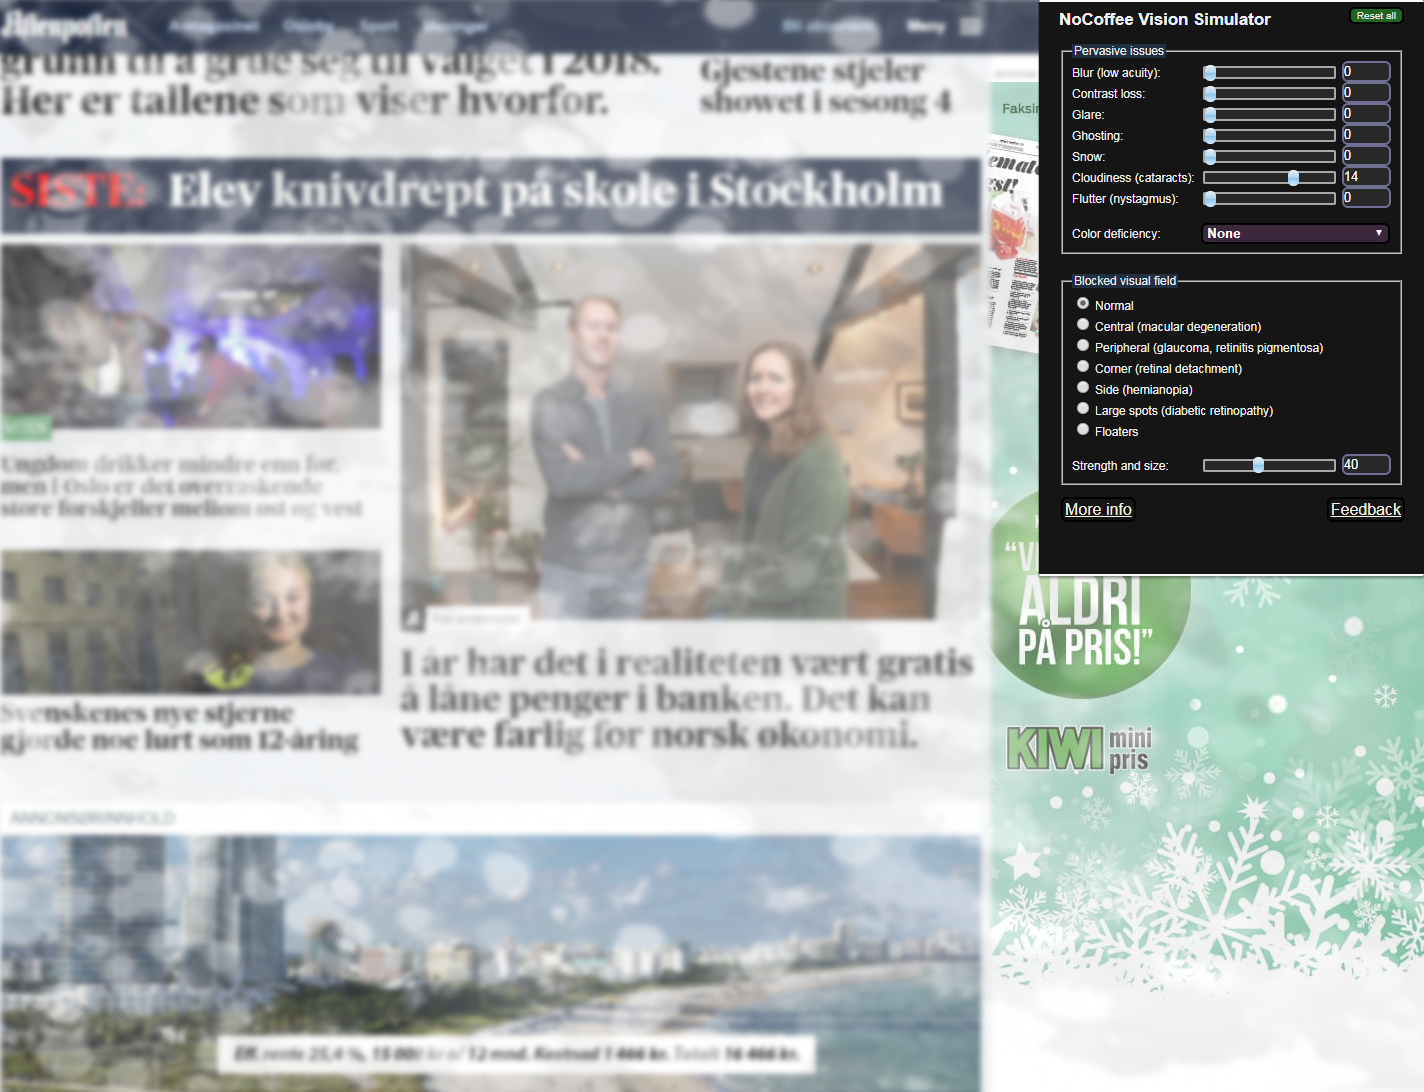
\includegraphics[width=\linewidth]{src/img/nocoffee.PNG}
%   \caption{The Chrome extension "NoCoffee" simulates different vision impairments by adding a filter on the screen.}\label{fig:nocoffee_browser_extension_discussion}
% \endminipage\hfill
% \end{figure}
% NoCoffee (see figure: \ref{fig:nocoffee_browser_extension_discussion}) simulates different impairments. There is nothing automatic about this tool, and it is up to the person performing the evaluation to decide whether a guideline is met or not. 

% Building on \textcite{bai_evaluation_2016}'s categories, I would therefore categorise accessibility evaluation methods as this:
% \begin{itemize}
%     \item Automatic and semi automatic tools
    
%     Tools that gives automatic feedback on whether a guideline is met or not. 
%     \item Empathy tools
    
%     Tools that can give an insight in how a UI can be experienced by people who has different impairments. This category includes software simulation tools and physical wearable simulation tools.
%     \item Expert testing
%     \item Testing with users
% \end{itemize}

% I have included empathy tools in this list because I do not think that these tools are automatic. These tools can either be used to empathise with users with impairments, or can be used as a quick test to see how a UI is experienced for people having different kinds of impairments.

% \section{Existing solutions}
% \subsection{Cambridge impairment simulation software}
% The simulator makes it possible to simulate different kinds of medical conditions, both affecting how digital information can be perceived visually and auditory. 

% However, the simulation has its flaws:
% \begin{itemize}
%     \item Outdated
    
%     The software itself is outdated and could not run on a modern macOS-computer. The Adobe Flash-version does work, but most tech-people would consider Flash outdated.
    
%     \item Minimal support for image files
    
%     Only a certain type of image files can be imported and used in the simulator.
    
%     \item Too technical
    
%     This simulator uses very technical terms on labels for different settings. For example is "Macular degeneration" used, which might give little meaning to a layman.
% \end{itemize}

% \subsection{NoCoffee browser extension}
% The simulator suffers from the same issues as the Cambridge simulation software in that it is outdated and too technical / medical. As one user of the simulator stated, it is hard to know which settings are realistic or makes sense for a person not familiar with vision impairments.

% \section{Developers view of Universal Design}
% In the focus group, the developers seemed to think of Universal Design as a requirement, most for people who makes websites in the public sector. Some developers seem to view Universal Design as being only for people with visual disabilities, and that alternative tags is the only tool web developers have to make a website universal designed.

% \section{Lack of education in Universal Design}
% In both the focus group, and according to a master thesis by Sanderengen (2017), there seem to be a lack of knowledge as to how you make ICT-solutions accessible in Norway. Some developers in Sanderengens study has learned about \gls{UniversalDesign} and WCAG success criterion by themselves, but this should be implemented in the IT-education. As one of the focus group participant stated, a good introduction at the start of the IT-education can help making it intuitive for developers and designers to use in projects from the start, rather than just something you include at the end of the project.